\documentclass[a4paper]{article}
\usepackage{tikz}
\usetikzlibrary{shapes.geometric}
\usetikzlibrary{positioning}
\usepackage{apacite}
\usepackage{tabularx}
\usepackage{siunitx}
\usepackage{amsmath}
\usepackage{rotating}
\usepackage{colortbl}
\usepackage{multirow}
\usepackage{arydshln} % Dashed hline
\usepackage{makecell} % Makecell
\usepackage{graphicx}
\usepackage[absolute]{textpos}

\sisetup{
    separate-uncertainty = true,
    table-align-uncertainty = true
}
% No more than 3000 words.


\begin{document}


\begin{titlepage}
    \title{\textbf{How does the hardness of water affect the rate of electrolysis? \\ \small Chemistry SL Internal Assesment}}
    \author{Zhou Changhui}
    \date{\today}
    \maketitle
    %\tableofcontents
\end{titlepage}

\section{Introduction and background knowledge}

Electrochemistry was not invented until the dawn of 1800s, marked by the creation of the first electrolytic cell by Alessandro Volta, and the subsequent discovery of water electrolysis by William Nicholson\cite{fabbrizzi2019strange}. Voltaic pile is considered the first artificial battery that provided continuous current to a circuit, laying a solid foundation for electricity-related studies. The discovery of water electrolysis by Nicholson, on the other hand, testified the composition of water and showed that water can be chemically decomposed. However, electrochemisty is still a relatively new subdiscipline in chemistry, and there are still many unknowns about the mechanism of electrolysis.

That work inspired Faraday's quantitative study on the general pattern of electrolysis, which resulted in Faraday's laws of electrolysis \cite{stock1991pathway}. Faraday concluded the amount of deposition is proportional to the amount of electric charge passing through the electrolyte, showing that electrolysis is foundamentally placing back of electrons. The study revealed the electric nature of many substances, formulated terms like ions, and greatly contributed to human's understanding of the submicroscopic world. 

Nowadays, electrolysis plays a vital role in chemical industry fields like metal refining, electroplating, and mass production of sodium and chloride. Water electrolysis is also currently the main method for the production of hydrogen and oxygen \cite{flowers-2019}.

Electrolysis experiments also serve a pivotal role in chemistry education, since it allows students to explore the property of different materials and reveal the atomic nature of substances (e.g. showing that water consists of hydrogen and oxygen atoms).

\textbf{Research question: How does the hardness of water (measured using MgCl$_2$ concentration) affect the rate of electrolysis?}

\section{Hypothesis and reasoning}



\section{Experiment design}

\subsection{Variables} 

\begin{itemize}
    \item Independent variable: hardness of water (manipulated using the concentration of MgCl$_2$: $0.2, 0.4, 0.6, 0.8$ and $ 1.0\SI{}{M}$).
    \item Dependent variable: Rate of electrolysis.
    \item Controlled variables: Temperature, atmospheric pressure, voltage, distance between electrodes, material of the electrodes and time duration of the experiment, etc. They are listed in Table \ref{tab.control}.
\end{itemize}

%Controlled variable table:
\begin{table}
    \centering
    \caption{Controlled variables}
    \label{tab.control}
    \begin{tabularx}{1.2\textwidth}{p{2cm} p{1cm} XX}
        \hline
        Variable                    & Value                  & Reason to control                                          & Method to control                                    \\ \hline
        Temperature              & $25^oC$                & Can significantly affect the rate of chemical reactions. & Complete the experiment during a short time period, in an air-conditioned room. \\
        Atmospheric pressure        & $\SI{1.0 }{atm}$       & Might change the volume and pressureof the gas collected      & Complete the experiment during a short time period. \\
        Voltage                     & $\SI{16 }{V}$          & Can affect the current passing through the electrolyte.                             & Use the same cell throughout the experiment. \\
        Distance between electrodes & $\SI{5.0}{cm}$        & Can affect the resistance between electrodes. & Use the same setup throughout the experiment. \\
        Material of the electrodes  & Graphite            & Can affect the conductivity and chemical property of the electrodes. & Use the same electrodes throughout the experiment. \\ 
        Time duration of the experiment & $\SI{20}{min}$ & Short time leads to inaccuarcy, but the concentration chage and side-effect accumulates over time. & Always time $\SI{20}{min}$ using a stopwatch.\\\hline
    \end{tabularx}
\end{table}

\subsection{Materials}

\begin{itemize}
    \item[*] 1 Iron stand with clamp ($\approx \SI{50}{cm}$)
    \item[*] 1 Side-armed U-shaped tube ($\approx \SI{100}{ml}$), with a pair of cork stoppers penetrated by graphite electrodes.
    \item[*] 1 Rubber tube.
    \item[*] 1 Gas syringe ($\approx \SI{20}{ml}$).
    \item[*] 1 Student power supply ($\approx \SI{16}{V}$) and conducting wire.
\end{itemize}

\subsection{Setup diagram}

\subsection{Procedure}

\begin{enumerate}
    \item Measure $m=\SI{2.06}{g}$ of MgCl${}_2\cdot 6$H${}_2$O in a beaker using analytical balance. Dissolve it with approximately $\SI{50}{ml}$ distilled water.
    \item Transfer the solution to a $\SI{100}{ml}$ volumetric flask. Rinse the beaker with distilled water and put it into the flask as well.
    \item Slowly add distilled water into the volumetric flask until it is just below the calibration mark. Use teat pipette to slowly add more distilled water until the base of the meniscus reaches the mark.
    \item Insert the stopper and invert the solution for multiple times to ensure solution homogeneity.
    \item Transfer the solution to the sidearmed U-shaped tube. Insert the corkstopper fitted with graphite electrodes and attach a syringe to one side arm using flexible tubing.
    \item Mark the meniscus in the U-shaped tube using thin marker pen.
    \item Switch the power supply to $\SI{16}{V}$ and turn it on. Start the timer at the same time.
    \item Keep adjusting the syringe to make sure the meniscus is on the marked line.
    \item Turn off the power supply when the timer reaches $\SI{20}{min}$.
    \item Repeat steps 1-9 twice to get two additional trials.
    \item Repeat steps 1-10 with $m=\SI{4.12}{g},\SI{6.18}{g},\SI{8.24}{g}$ and $\SI{10.30}{g}$.
\end{enumerate}

\section{Results}

\subsection{Raw data}

\begin{table}[ht]
\centering
\caption{Raw data}
\begin{tabular}{cccccc}
    \hline
    \makecell{Experi-\\ ment No.} & Trial & {Mass (\si{\gram})} & \makecell{Solution\\ Volume (\si{\milli\litre})} & \makecell{Gas Volume\\ (\si{\milli\litre})} & {Time (\si{\second})} \\
    \hline
    1 & 1 & $4.0920 \pm 0.0001$  & $100.0 \pm 0.5$ &  $4.2 \pm 0.1$ & $1200 \pm 1$ \\
    1 & 2 & $4.0593 \pm 0.0001$  & $100.0 \pm 0.5$ &  $3.9 \pm 0.1$ & $1200 \pm 1$ \\
    1 & 3 & $4.0300 \pm 0.0001$  & $100.0 \pm 0.5$ &  $3.2 \pm 0.1$ & $1200 \pm 1$ \\
    2 & 1 & $8.1372 \pm 0.0001$  & $100.0 \pm 0.5$ &  $6.9 \pm 0.1$ & $1200 \pm 1$ \\
    2 & 2 & $8.1031 \pm 0.0001$  & $100.0 \pm 0.5$ &  $7.0 \pm 0.1$ & $1200 \pm 1$ \\
    2 & 3 & $8.1203 \pm 0.0001$  & $100.0 \pm 0.5$ &  $7.1 \pm 0.1$ & $1200 \pm 1$ \\
    3 & 1 & $12.1982 \pm 0.0001$ & $100.0 \pm 0.5$ & $10.0 \pm 0.1$ & $1200 \pm 1$ \\
    3 & 2 & $12.2637 \pm 0.0001$ & $100.0 \pm 0.5$ & $10.0 \pm 0.1$ & $1200 \pm 1$ \\
    3 & 3 & $12.1816 \pm 0.0001$ & $100.0 \pm 0.5$ & $10.0 \pm 0.1$ & $1200 \pm 1$ \\
    4 & 1 & $16.2455 \pm 0.0001$ & $100.0 \pm 0.5$ & $12.9 \pm 0.1$ & $1200 \pm 1$ \\
    4 & 2 & $16.2241 \pm 0.0001$ & $100.0 \pm 0.5$ & $12.8 \pm 0.1$ & $1200 \pm 1$ \\
    4 & 3 & $16.2502 \pm 0.0001$ & $100.0 \pm 0.5$ & $13.0 \pm 0.1$ & $1200 \pm 1$ \\
    5 & 1 & $20.1607 \pm 0.0001$ & $100.0 \pm 0.5$ & $14.1 \pm 0.1$ & $1200 \pm 1$ \\
    5 & 2 & $20.3037 \pm 0.0001$ & $100.0 \pm 0.5$ & $14.9 \pm 0.1$ & $1200 \pm 1$ \\
    5 & 3 & $20.3013 \pm 0.0001$ & $100.0 \pm 0.5$ & $14.3 \pm 0.1$ & $1200 \pm 1$ \\
    \hline
\end{tabular}
\end{table}




\subsection{Processed data}

Processed data can be found in Table \ref{tab.proc}. The rate is plotted against the MgCl$_2$ concentration, and the graph is plotted in Figure \ref{fig.proc}.

\begin{table}[h!]
\centering
\caption{Processed data}
\label{tab.proc}
\begin{tabular}{cc}
\hline
\makecell{MgCl$_2$ concentration\\ (mol L$^{-1}$)} & \makecell{Rate of electro-\\lysis ($10^{-7}$ mol s$^{-1}$)} \\

\hline
0.200$\pm$0.002 & 1.367$\pm$0.051 \\
0.399$\pm$0.001 & 2.392$\pm$0.034 \\
0.601$\pm$0.002 & 3.405$\pm$0.017 \\
0.799$\pm$0.001 & 4.408$\pm$0.034 \\
0.996$\pm$0.004 & 4.931$\pm$0.137 \\
\hline
\end{tabular}
\end{table}

\begin{figure}
    \centering
    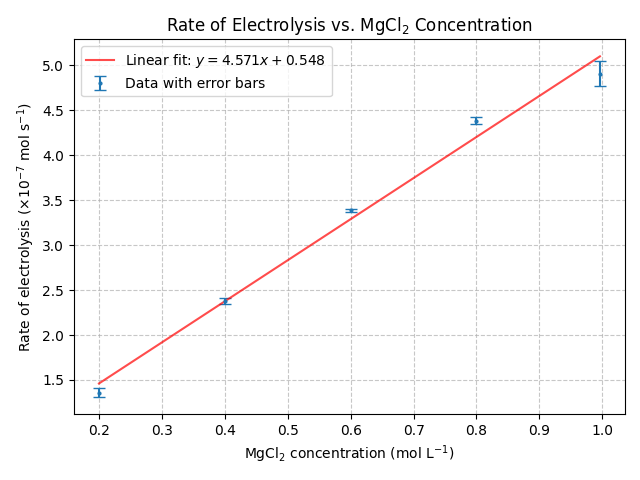
\includegraphics[width=\textwidth]{fit.png}
    \caption{Rate of electrolysis against MgCl$_2$ concentration}
    \label{fig.proc}
\end{figure}


\subsection{Sample processing}

\section{Discussion and conclusion}

The diagram suggests strong correlation between the rate and the concentration. The best fit line has 

\begin{itemize}
    \item a gradient of $4.591 \times 10^{-7}\SI{}{L s^{-1}}$
    \item and a y-intercept of $0.550\times 10^{-7} \SI{}{mol s^{-1}}$.
\end{itemize}

The error on the independent variable was too insignificant to be shown on the graph. The errorbar on the y-axis is relatively small, showing high precision of the experiment.

The dots and error bars shows strong linear relationship between the rate and the concentration, which can be quantified with a high r$^2$ value of $0.989032$. The linear correlation suggests that the initial hypothesis is valid.

Not all the error bars are passed through by the best fit line. This might have resulted from the high concentration of the last several groups of trials. As is mentioned in the hypothesis part, high concentration can change the behaviour of the electrolyte and cause side reaction. This will be further discussed in Section \ref{sec.eval}.

\section{Evaluation}
\label{sec.eval}

The experiment was conducted successfully, providing sufficient data supporting the initial hypothesis. However, the expected deviation from linear relationship is not signifcant in the data. There is still room for improvement.

\begin{itemize}
    \item Imprecise marking: thin marker pen is used to mark the meniscus of the initial solution, which still results in a relatively thick stroke that can lead to unexpected uncertainty. Using a graduated, thin glass ware instead can minimize the uncertainty from adjustment.
    \item High concentration: a concentration higher than general cases where water electrolysis take place is adopted, due to the limited time and apparatus in the laboratory. That resulted in side reaction, like the production of chlorine taking place. Using more dilute solution, larger electrode and longer experiment time can help stop the side reaction.
    \item Bubbles' adhesion to electrodes: some gas produced is observed to have delayed or no detachment to the carbon electrodes. This can cause underming of the total gas production, 
\end{itemize}

\bibliographystyle{apacite}
\bibliography{cit.bib}

\end{document}